% ====== TAREA 1 MATEMATICAS APLICADAS ======

\documentclass{article}
\usepackage[utf8x]{inputenc}
\usepackage[spanish]{babel}
\usepackage{cancel}
\usepackage{amsmath}
\usepackage{mathtools}
\usepackage{amsfonts}
\usepackage{amssymb}
\usepackage{graphicx}
\usepackage{enumitem}
\usepackage[usenames]{color}
\usepackage[text={20cm,25cm},centering,top=1.5cm,bottom=1.5cm,letterpaper,showframe=false]{geometry}
\renewcommand{\baselinestretch}{1.5}
\parindent  = 0mm
\parskip    = 4mm
\definecolor{azul}{RGB}{10,80,190}
\definecolor{negro}{RGB}{0,0,0}
\definecolor{rojo}{RGB}{190,80,10}
\definecolor{verde}{RGB}{0,120,50}

\begin{document}
    \title{Tarea 1}
    \author{Careaga Carrillo Juan Manuel \\ Quiróz Castañeda Edgar \\ Soto Corderi Sandra del Mar}
    \date{Lunes 21 de Septiembre del 2018}
    \maketitle

	\begin{enumerate}
   	% Ejercicio 1
   	\item {
        Dibujar la región $W$ definida por las superficies $x + 2y + 3z = 6$,
        $x = 0$, $y = 0$ y $z = 0$.
        Expresar la integral triple $\iiint_Wf(x,y,z)dV$ de las seis formas posibles
        como integrales iteradas.

        \color{azul}
				La región morada es el plano $x + 2y + 3z = 6$, la roja el plano
				$x = 0$, la azul $z = 0$ y la verde $y = 0$.

				\begin{center}
            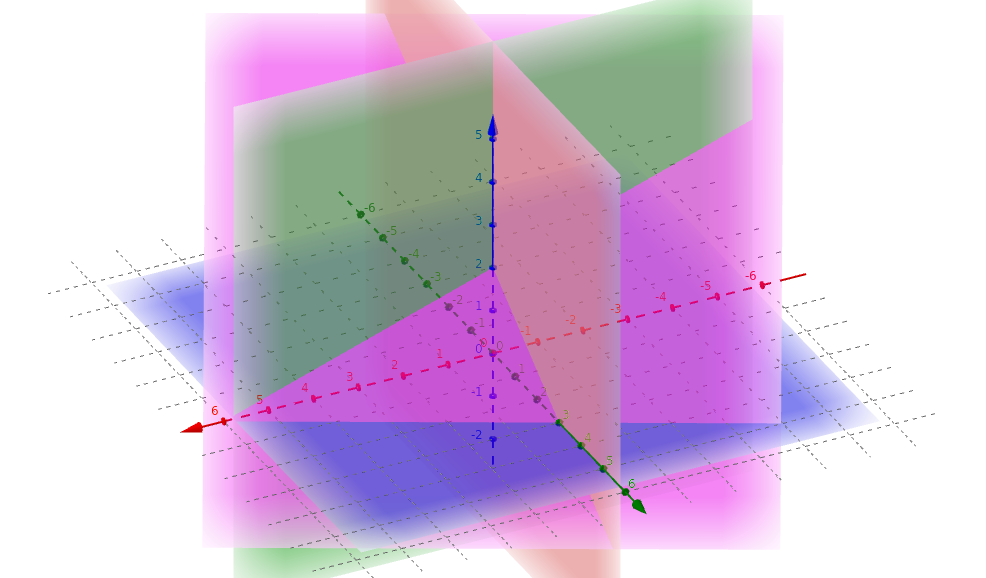
\includegraphics[width=6cm]{img/ej1.png}
        \end{center}

				Tomemos por ejemplo la triple integral en la que primero se integra sobre la
				variable $x$, luego sobre $y$ y al final sobre $z$.\\
				En general, tenemos que los límites que se obtienen despejando la
				variable de $x + 2y + 3z = 6$ son positivos y como el otro límite es 0,
				entonces podemos saber cuál es el límite superior y cual es el inferior.

				Para la primera integral, hay definir los límites despejando $x$ de las
				superficies que limitan la región.\\
				Es decir $x = 0$ y $x + 2y + 3z = 6 \implies x = 6 - 2y - 3z$.
				\[\int_{0}^{6-2y-3z} dx\]
				Después, hay que hacer lo mismo con la variable $y$, suponiendo a $x$
				como nula, pues ya se ha integrado, es decir $y = 0$ y
				$6 = 0 + 2y + 3z \implies y = 3- \frac{3}{2}dz$.
				\[\int_{0}^{3-\frac{3}{2}z} dy\]
				Finalmente, hay que hacer lo mismo para $z$, esto es $z = 0$ y
				$6 = 0 + 0 + 3z \implies z = 2$.
				\[\int_{0}^{2} dz\]
				Entonces, la primera triple integral sería
				\[\int_{0}^{2} \int_{0}^{3-\frac{3}{2}z} \int_{0}^{6-2y-3z} dxdydz\]
				Análogamente, cambiando el orden de integración de las variables, se
				obtienen las demás posibles integrales triples.
				Estas son
        \begin{align*}
            &\int_{0}^{3} \int_{0}^{2-\frac{2}{3}y} \int_{0}^{6-2y-3z} dxdzdy\\
            &\int_{0}^{2} \int_{0}^{6-3z} \int_{0}^{3-\frac{x+3z}{2}} dydxdz\\
            &\int_{0}^{6} \int_{0}^{2-\frac{x}{3}} \int_{0}^{3-\frac{x+3z}{2}} dydzdx\\
            &\int_{0}^{6} \int_{0}^{3-\frac{x}{2}} \int_{0}^{2-\frac{x+2y}{3}} dzdydx\\
            &\int_{0}^{3} \int_{0}^{6-2y} \int_{0}^{2-\frac{x+2y}{3}} dzdxdy
        \end{align*}

	}

	% Ejercicio 2
    \item {
        Dibujar la región W descrita por la integral iterada
        \[
            \int_{0}^{1} \int_{z^3}^{\sqrt{z}} \int_{0}^{4-x} dydxdz
        \]
        Calcular su volumen.

        \color{azul}

				El dibujo de la región sería la superposición de las regiones en el
				intervalo en $z$ de 0 a 1.
				\begin{center}
            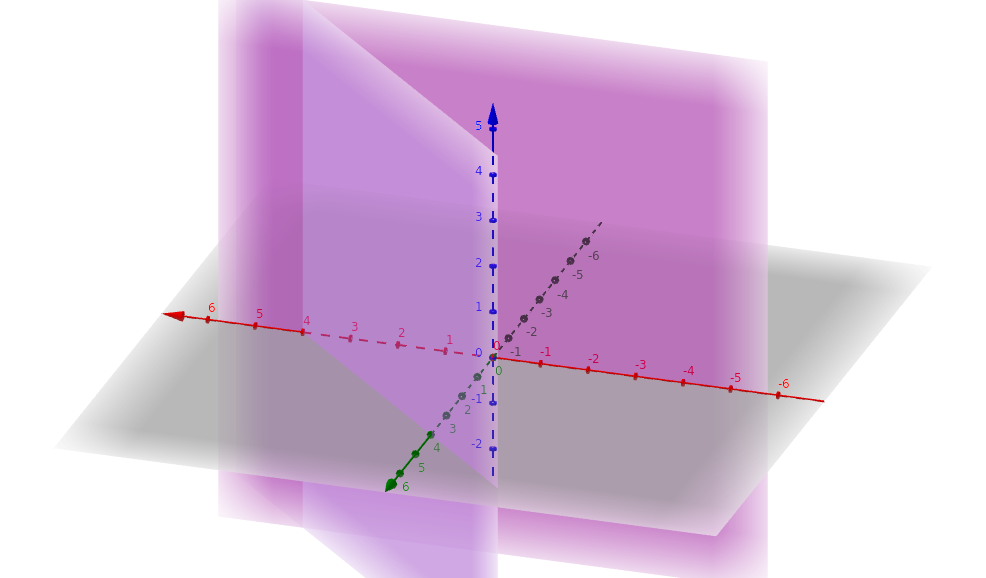
\includegraphics[width=6cm]{img/ej2_1.png}
						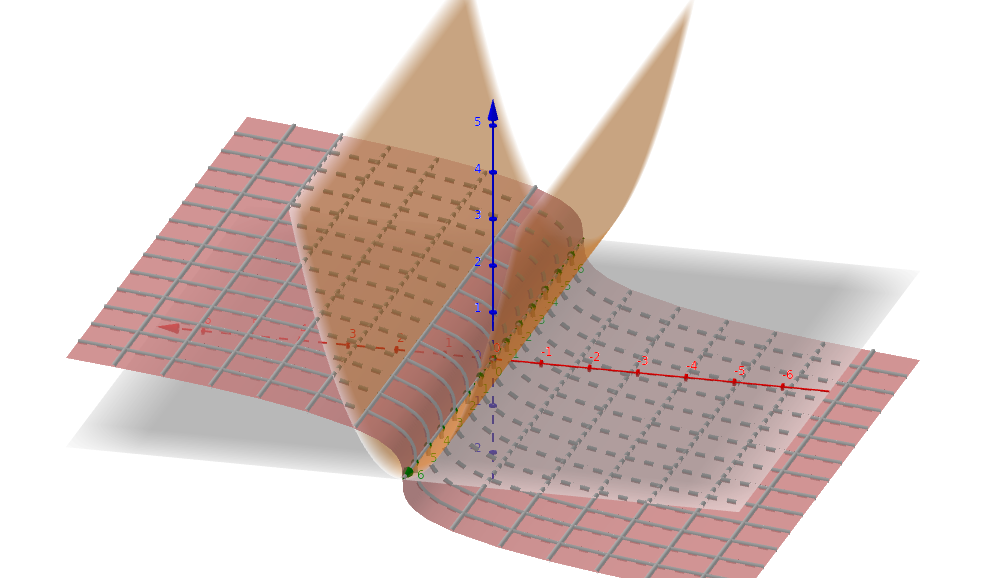
\includegraphics[width=6cm]{img/ej2_2.png}
        \end{center}

        \begin{align*}
            \int_{0}^{1} \int_{z^3}^{\sqrt{z}} \int_{0}^{4-x} dydxdz
                &= \int_{0}^{1} \int_{z^3}^{\sqrt{z}} y \Big|_{0}^{4-x} dxdz
                    = \int_{0}^{1} \int_{z^3}^{\sqrt{z}} ((4-x)-0) dxdz
                    = \int_{0}^{1} \int_{z^3}^{\sqrt{z}} (4-x) dxdz\\
                &= \int_{0}^{1} (4x - \frac{1}{2}x^2) \Big |_{z^3}^{\sqrt{z}} dz
                    = \int_{0}^{1} (4(z^{\frac{1}{2}}) - \frac{1}{2}(z^{\frac{1}{2}})^2) - (4(z^3)
                    - \frac{1}{2}(z^3)^2) dz\\
                &= \int_{0}^{1} (4z^{\frac{1}{2}} - \frac{1}{2}z - 4z^3 + \frac{1}{2}z^6) dz
                    = (\frac{8}{3}z^{\frac{3}{2}} - \frac{1}{4}z^2 - z^4 + \frac{1}{14}z^7) \Big |_{0}^{1}\\
                &= (\frac{8}{3}(1)^{\frac{3}{2}} - \frac{1}{4}(1)^2 - (1)^4 + \frac{1}{14}(1)^7)
                    - (\frac{8}{3}(0)^{\frac{3}{2}} - \frac{1}{4}(0)^2 - (0)^4 + \frac{1}{14}(0)^7)\\
                &= \frac{8}{3} - \frac{1}{4} - 1 + \frac{1}{14} = \frac{32-3}{12} - 1 + \frac{1}{14}
                    = \frac{203+6}{84} - 1 = \frac{209 - 84}{84} = \frac{125}{84}
        \end{align*}
    }

    % Ejercicio 3
    \item {
        Integrar la función $f(x,y) = x^2 + 2xy^2 + 2$ sobre la región $D$
        acotada por la gráfica de $y = -x^2 + x$, el eje $x$, y las rectas
        $x = 0$ y $x = 2$.

        \color{azul}
        \[
            -x^2 + x = 0 \implies x = x^2 \implies x = 1, 0
        \]
        \begin{align*}
            -(0.5)^2 + 0.5 = -0.25 + 0.5 & = 0.25 > 0 \\
            -(1.5)^2 + 1.5 = -2.25 + 1.5 & = -0.75 < 0
        \end{align*}
        Entones la función es positiva en $(0, 1)$ y negativa en $(1, 2]$.

        Por lo tanto hay que considerar dos integrales para calcular el volumen deseado.
        \begin{align*}
            &  \int_{0}^{1} \int_{0}^{-x^2+x} (x^2 + 2xy^2 + 2) dy dx + \int_{1}^{2} \int_{-x^2+x}^{0} (x^2 + 2xy^2 + 2) dy dx\\
            &= \int_{0}^{1} (x^2y + \frac{2}{3}xy^3 + 2y) \Big |_{0}^{-x^2+x}dx + \int_{1}^{2} (x^2y + \frac{2}{3}xy^3 + 2y) \Big |_{-x^2+x}^{0}dx\\
            &= \int_{0}^{1} (x^2(-x^2+x) + \frac{2}{3}x(-x^2+x)^3 + 2(-x^2+x)) - (x^2(0) + \frac{2}{3}x(0)^3 + 2(0))dx\\
            &+ \int_{1}^{2} (x^2(0) + \frac{2}{3}x(0)^3 + 2(0)) -  (x^2(-x^2+x) + \frac{2}{3}x(-x^2+x)^3 + 2(-x^2+x))dx\\
            &= \int_{0}^{1} (x^2(-x^2+x) + \frac{2}{3}x(-x^2+x)^3 + 2(-x^2+x))dx + \int_{1}^{2}-(x^2(-x^2+x) + \frac{2}{3}x(-x^2+x)^3 + 2(-x^2+x))dx\\
            &= \int_{0}^{1} (-x^4+x^3 + \frac{2}{3}(-x^7 + x^6 - x^5 + x^4) - 2x^2 + 2x)dx - \int_{1}^{2} (-x^4+x^3 + \frac{2}{3}(-x^7 + x^6 - x^5 + x^4) - 2x^2 + 2x)dx\\
            &= \int_{0}^{1} (-\frac{1}{3}x^4+x^3 + \frac{2}{3}(-x^7 + x^6 - x^5) - 2x^2 + 2x)dx - \int_{1}^{2} (-\frac{1}{3}x^4+x^3 + \frac{2}{3}(-x^7 + x^6 - x^5) - 2x^2 + 2x)dx\\
            &= (-\frac{1}{15}x^5 + \frac{1}{4}x^4 + \frac{2}{3}(-\frac{1}{8}x^8 + \frac{1}{7}x^7 - \frac{1}{6}x^6) - \frac{2}{3}x^3 + x^2) \Big |_{0}^{1}
            - (-\frac{1}{15}x^5 + \frac{1}{4}x^4 + \frac{2}{3}(-\frac{1}{8}x^8 + \frac{1}{7}x^7 - \frac{1}{6}x^6) - \frac{2}{3}x^3 + x^2) \Big |_{1}^{2}\\
            &=(-\frac{1}{15} + \frac{1}{4} + \frac{2}{3}(-\frac{1}{8} + \frac{1}{7} - \frac{1}{6} - 1) + 1)
            -  ((-\frac{1}{15}(2)^5 + \frac{1}{4}(2)^4 + \frac{2}{3}(-\frac{1}{8}(2)^8 + \frac{1}{7}(2)^7 - \frac{1}{6}(2)^6 - 2^3) + (2)^2)\\
            &- (-\frac{1}{15} + \frac{1}{4} + \frac{2}{3}(-\frac{1}{8} + \frac{1}{7} - \frac{1}{6} - 1) + 1))\\
            &= (\frac{15 - 4}{60} + \frac{2}{3}(\frac{-42+48-56-336}{336}) + 1)
            -((-\frac{32}{15} + \frac{16}{4} + \frac{2}{3}(-\frac{256}{8} + \frac{128}{7} - \frac{64}{6} - 8) + 4) \\
            &-(\frac{15 - 4}{60} + \frac{2}{3}(\frac{-42+48-56-336}{336}) + 1))\\
            &= 2(\frac{11}{60} + \frac{2}{3} \cdot \frac{-382}{336} + 1) - (-\frac{32}{15} + 4 + \frac{2}{3}(-32 + \frac{128}{7} - \frac{32}{3} - 8) + 4)\\
            &= 2(\frac{11}{60} - \frac{382}{504} + 1) - (-\frac{32}{15} + 8 + \frac{2}{3}(-40 + \frac{384-224}{21}))\\
            &= 2(\frac{462 - 1910}{2520} + 1) - (-\frac{32}{15} + 8 + \frac{2}{3} \cdot \frac{160-840}{21})\\
            &= 2(\frac{-1448 + 2520}{2520}) - (-\frac{32}{15} + 8 + \frac{2}{3} \cdot \frac{-680}{21}) = 2 \cdot \frac{1072}{2520} - (-\frac{32}{15} + 8 - \frac{1360}{63})\\
            &= \frac{1072}{1260} - (\frac{-672-6800}{315} + 8) = \frac{1072}{1260} - (\frac{-7472+2520}{315})\\
            &= \frac{1072}{1260} - (-\frac{4952}{315}) = \frac{1072}{1260} + \frac{4952}{315} = \frac{1072+19808}{1260} = \frac{20880}{1260} \approx 16.6
        \end{align*}
    }

	% Ejercicio 4
    \item {
        Usar integrales dobles para calcular el área de una elipse con semiejes $a$ y $b$.

        \color{azul}
        Supongamos, sin perder la generalidad, que $a\geq b$. La ecuación canónica de la elipse horizontal cuyo centro está en el origen del plano y tiene semiejes $a$ y $b$ es
        \[
            \frac{x^2}{a^2}+\frac{y^2}{b^2}=1
        \]
        Equivalentemente, podemos afirmar entonces que
        \(\displaystyle
            y=\frac{\pm\sqrt{a^2 b^2 -b^2 x^2}}{a}
        \)
        describe nuestro lugar geométrico. Por simpleza, y aprovechando su simetría con los ejes $X$ e $Y$, dividimos la elipse en 4 regiones iguales delimitadas por los ejes coordenados y únicamente calcularemos el área de una de ellas, llámese $R$, al final, el área total se obtendrá de multiplicar el área de dicha región por 4.
        \begin{center}
            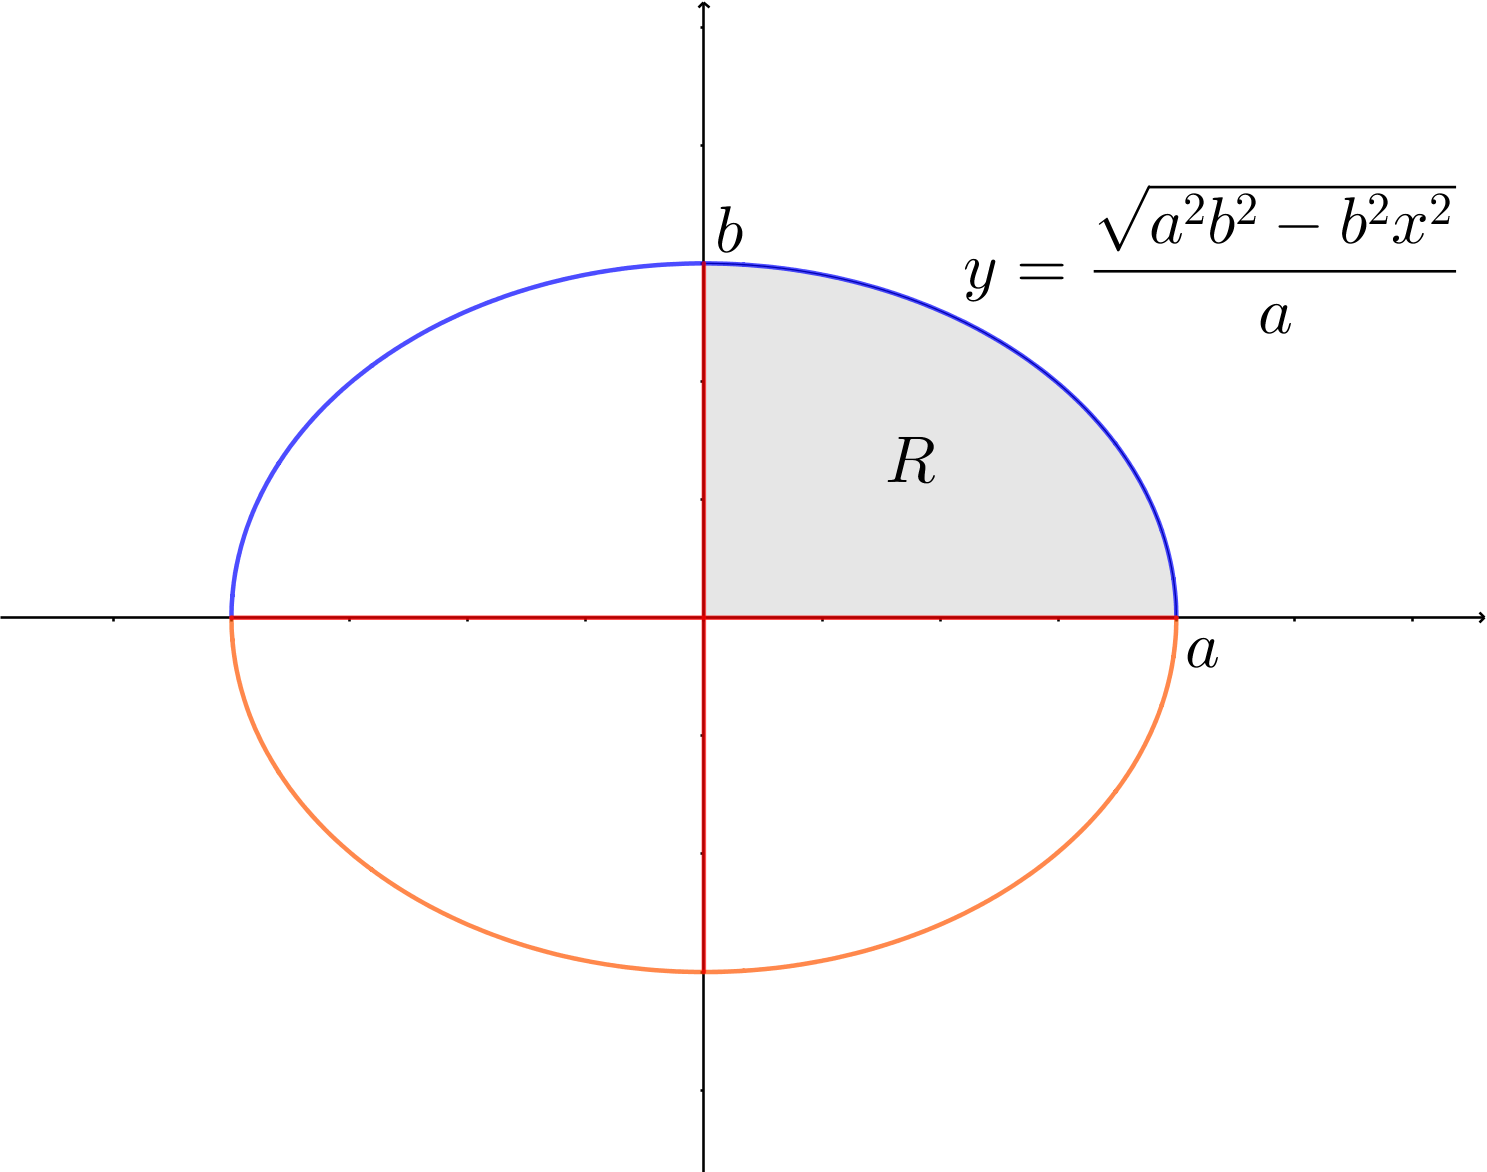
\includegraphics[width=6cm]{img/ej4.png}
        \end{center}
        $R$ es una región $y-$simple, por lo que
        \(\displaystyle
            R=\left\{
                (x,y)\,\bigg\vert\,
                0\leq x\leq a;
                0\leq y\leq\frac{\sqrt{a^2b^2-b^2x^2}}{a}
            \right\}
        \)
        , entonces el área de $R$ está dada por
        \[
            \iint_R{dA}
            =\int_0^a{\int_0^{ \frac{\sqrt{a^2b^2-b^2x^2}}{a} }{dy}\,dx}
            =\int_0^a{\frac{1}{a}\sqrt{a^2b^2-b^2x^2}\,dx}
            =\frac{b}{a}\int_0^a{\sqrt{a^2-x^2}\,dx}
        \]
        Haciendo la sustitución $x=a \sen{\theta}$ con $0\leq\theta\leq\frac{\pi}{2}$, tenemos que $dx=a\cos{\theta}\,d\theta$; para los límites de la integral, si $x=0=a\sen{\theta}$ entonces $\theta=0$ y si $x=a=a\sen{\theta}$, entonces $\theta=\frac{\pi}{2}$. La integral queda como
        \[
            \frac{b}{\cancel{a}}\int_0^{\frac{\pi}{2}}{
                \sqrt{a^2-a^2\sen^2{\theta}}\,\cancel{a}\cos{\theta}\,d\theta
            }
            =b\int_0^{\frac{\pi}{2}}{
                \sqrt{a^2(1-\sen^2{\theta})}\cos{\theta}\,d\theta
            }
            =ab\int_0^{\frac{\pi}{2}}{
                \cos^2{\theta}\,d\theta
            }
        \]
        Usando la fórmula del ángulo doble para el coseno tenemos
        \[
            =ab\int_0^\frac{\pi}{2}{
                \frac{1}{2}(1+\cos{(2\theta)})
            \,d\theta}
            =\frac{ab}{2}\left[
                \theta + \frac{1}{2}\sen{(2\theta)}
            \right]_0^\frac{\pi}{2}
            =\frac{ab}{2}\left[
                \frac{\pi}{2}+0
            \right]
            =\frac{\pi ab}{4}
        \]
        Por lo tanto, el área de la elipse es 4 veces lo anterior, es decir $A=\pi ab$
	}

	% Ejercicio 5
    \item {
        Mostrar que al evaluar $\iint_DdA$, donde $D$ es una región $y$-simple, se reproduce la fórmula del cálculo de una variable para el área entre dos curvas.

        \color{azul}
        Sea $D$ una región $y-$simple, entonces de define como
        \(
            D=\left\{
                (x,y)\,\bigg\vert\, a\leq x\leq b;\;
                \varphi_1(x)\leq y\leq\varphi_2(x)
            \right\}
        \)
        para algunos $a,b\in\mathbb{R}$ y $\varphi_1(x):\mathbb{R}\rightarrow\mathbb{R}$, $\varphi_2(x):\mathbb{R}\rightarrow\mathbb{R}$. Entonces
        \[
            \iint_D{dA}
            =\int_a^b{
                \int_{\varphi_1(x)}^{\varphi_2(x)}{dy}
            \,dx}
        \]
        por el Teorema de Fubini
        \[
            =\int_a^b{
                \left[ y \right]_{\varphi_1(x)}^{\varphi_2(x)}
            \,dx}
            =\int_a^b{
                \left[ \varphi_2(x) - \varphi_1(x) \right]
            \,dx}
            =\int_a^b{\varphi_2(x)\,dx}
            -\int_a^b{\varphi_1(x)\,dx}
        \]
        que es como se calcula el área comprendida entre las curvas $\varphi_1(x)$ y $\varphi_2(x)$ en el intervalo $[a,b]$.
    }

	% Ejercicio 6
    \item {
        Describir la región que se encuentra entre el cono $z = \sqrt{x^2 + y^2}$ y el paraboloide $z=x^2+y^2$ como una región elemental.

        \color{azul}
        Se puede cracterizar como una región de tipo III. Proyectando las gráficas al plano $yz$ tenemos
        \begin{center}
            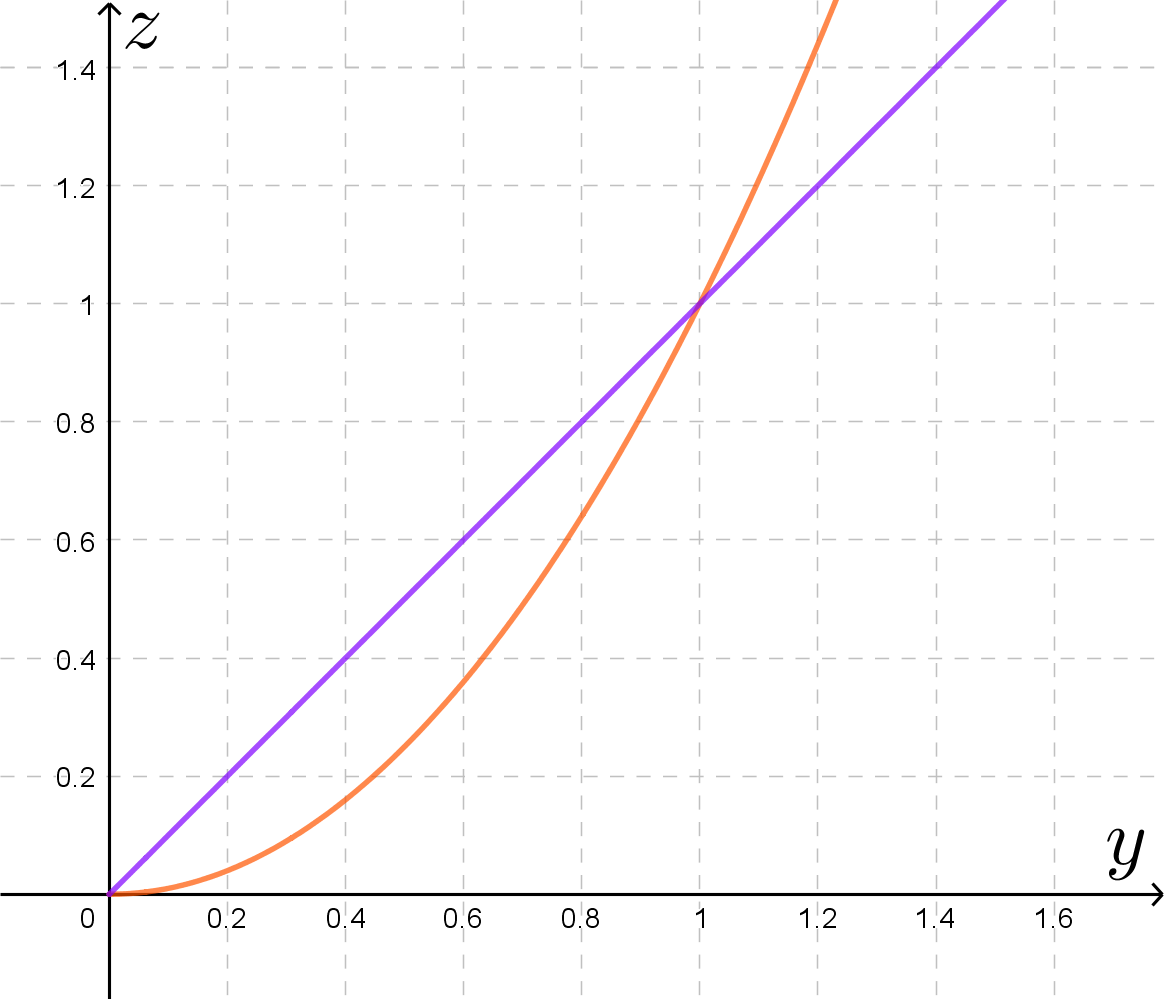
\includegraphics[width=6cm]{img/ej6.png}
        \end{center}
        Como estamos en el plano $yz$, entonces $x=0$ y las ecuaciones se convertirían en
        \begin{eqnarray*}
            z=y\\
            z=y^2
        \end{eqnarray*}
        Al igualar ambas ecuaciones encontraremos sus intersecciones
        \begin{eqnarray*}
            y=y^2\\
            \therefore \{y=0, y=1\}
        \end{eqnarray*}
        Y si de las ecuaciones originales despejamos la $x$ nos quedaría
        \begin{eqnarray*}
            x=\sqrt{z^2-y^2}\\
            x=\sqrt{x-y^2}
        \end{eqnarray*}
        Por lo que la descripción de la región, por lo menos en el primer octante, queda como
        \[
            R_1=\left\{
                    (x,y,z)\,\big\vert\,
                    \sqrt{z-y^2}\leq x\leq\sqrt{z^2-y^2};\,
                    0\leq y\leq 1;\,
                    y^2\leq z\leq y
                \right\}
        \]
        Debido a las simetrías que presentan ambas gráficas con los planos $xz$ e $yz$, encontrar la descripción en los octantes restanes debe ser sencillo.

        Para el segundo octante el comportamento en $y$ y en $z$ es idéntico, sólo reflejamos en $x$
        \[
            R_2=\left\{
                    (x,y,z)\,\big\vert\,
                    -\sqrt{z^2-y^2}\leq x\leq-\sqrt{z-y^2};\,
                    0\leq y\leq 1;\,
                    y^2\leq z\leq y
                \right\}
        \]
        Para el tercer octante reflejamos $x$ y reflejamos $y$ (con respecto a $R_1$)
        \[
            R_3=\left\{
                    (x,y,z)\,\big\vert\,
                    -\sqrt{z^2-y^2}\leq x\leq-\sqrt{z-y^2};\,
                    -1\leq y\leq 0;\,
                    y^2\leq z\leq y
                \right\}
        \]
        Y para el cuarto octante sólo reflejamos $y$ (de nuevo, es con respecto a $R_1$)
        \[
            R_4=\left\{
                    (x,y,z)\,\big\vert\,
                    \sqrt{z-y^2}\leq x\leq\sqrt{z^2-y^2};\,
                    -1\leq y\leq 0;\,
                    y^2\leq z\leq y
                \right\}
        \]
        Al final, la región comprendida entre ambas superficies es la unión de estas 4 regiones (pues no existe la gráfica en los octantes 5, 6, 7, u 8).
        \[
            R=\bigcup_{i=1}^4{R_i}
        \]
    }

    % Ejercicio 7
    \item {
        Hallar el volumen acotado por el paraboloide $z = 2x^2 + y^2$ y el cilindro $z = 4 - y^2$\\

        \color{azul}
        Para calcular el volumen tendríamos $\iiint_W dV$.

        Primero veamos la intersección de las dos superficies como: $4-y^2 = 2x^2 + y^2 \Rightarrow x^2+y^2 = 2$

        La intersección del paraboloide y el cilindro se ve :
        \begin{center}
            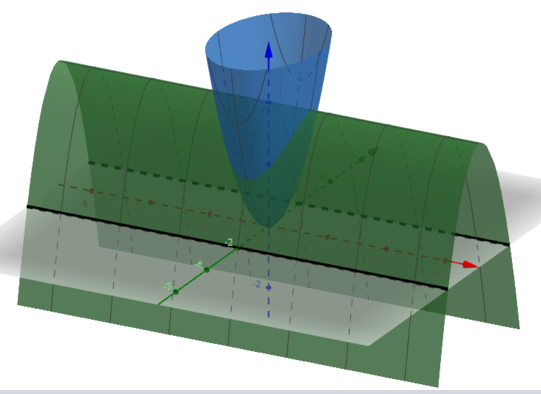
\includegraphics[width=7cm]{img/ejercicio7.png}
        \end{center}
        La proyección del volumen en el plano $xy$ se ve como:
        \begin{center}
            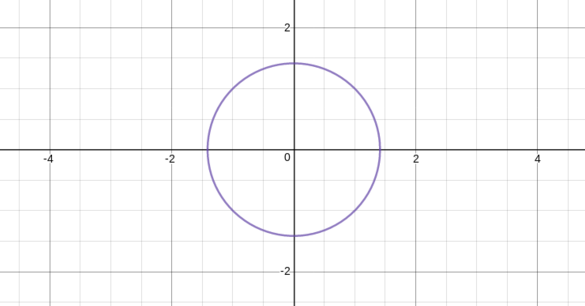
\includegraphics[width=7cm]{img/ejercicio71.png}\\
        \end{center}
        De ahí, caracterizamos el volumen como: $\displaystyle\int_{-\sqrt{2}}^{\sqrt{2}}\int_{-\sqrt{2-x^2}}^{\sqrt{2-x^2}}\int_{2x^2+y^2}^{4-y^2}dzdydx$

        Resolviendo la integral triple tenemos:
        \begin{align*}
            \displaystyle
            &\int_{2x^2+y^2}^{4-y^2}dz = z\Bigm|_{2x^2+y^2}^{4-y^2} = 4-y^2-2x^2-y^2 = -2y^2-2x^2+4\\
            &\int_{-\sqrt{2-x^2}}^{\sqrt{2-x^2}} (-2y^2-2x^2+4)dy = \int_{-\sqrt{2-x^2}}^{\sqrt{2-x^2}} (-2y^2)dy +  \int_{-\sqrt{2-x^2}}^{\sqrt{2-x^2}} (-2x^2)dy + \int_{-\sqrt{2-x^2}}^{\sqrt{2-x^2}} (4)dy\\
            &\int_{-\sqrt{2-x^2}}^{\sqrt{2-x^2}} (-2y^2-2x^2+4)dy = (-\frac{2}{3}y^3)\Bigm|_{-\sqrt{2-x^2}}^{\sqrt{2-x^2}} + (-2x^2y)\Bigm|_{-\sqrt{2-x^2}}^{\sqrt{2-x^2}} + (4y)\Bigm|_{-\sqrt{2-x^2}}^{\sqrt{2-x^2}}\\
            &\int_{-\sqrt{2-x^2}}^{\sqrt{2-x^2}} (-2y^2-2x^2+4)dy = -\frac{4(\sqrt{2-x^2})^3}{3} -4x^2\sqrt{2-x^2} + 8\sqrt{2-x^2}\\
            &\int_{-\sqrt{2}}^{\sqrt{2}}(-\frac{4(\sqrt{2-x^2})^3}{3} -4x^2\sqrt{2-x^2} + 8\sqrt{2-x^2})dx = \int_{-\sqrt{2}}^{\sqrt{2}}(-\frac{4(\sqrt{2-x^2})^3}{3})dx + \int_{-\sqrt{2}}^{\sqrt{2}}(-4x^2\sqrt{2-x^2})dx+ \int_{-\sqrt{2}}^{\sqrt{2}}(8\sqrt{2-x^2})dx\\
            &\int_{-\sqrt{2}}^{\sqrt{2}}(-\frac{4(\sqrt{2-x^2})^3}{3})dx = \frac{4}{3}\int_{-\sqrt{2}}^{\sqrt{2}}(2-x^2)^{-\frac{3}{2}} dx
        \end{align*}
        Usando integración por sustitución $z = \frac{u}{2}$:
        $= \frac{4}{3}\cdot\frac{1}{16}\int(8-u^2)^{-\frac{3}{2}} du $\\
        Usando integración por partes: $u = (8-u^2)^{-\frac{3}{2}} , dv = 1$:
        $\frac{4}{3}\cdot\frac{1}{16}(u)(8-u^2)^{-\frac{3}{2}} + \int3u^2\sqrt{8-u^2}du$\\
        Usando integración por sustitución $u = 2\sqrt{2}\sen(m)$ $\int3u^2\sqrt{8-u^2}du = 3 \cdot 16\sqrt{2} \int \sen^2(m)\cos(m)\sqrt{8-8\sen^2(m)}$\\
        Simplificando y regresando la u:$\int3u^2\sqrt{8-u^2}du = -24(\arcsen(\frac{1}{2\sqrt{2}}u) - \frac{1}{4}\sen(4\arcsen(\frac{1}{2\sqrt{2}}u)))$\\
        De ahí, $\frac{4}{3}\cdot\frac{1}{16}\int(8-u^2)^{-\frac{3}{2}} du = \frac{4}{3}\cdot\frac{1}{16}(u)(8-u^2)^{-\frac{3}{2}} -24(\arcsen(\frac{1}{2\sqrt{2}}u) - \frac{1}{4}\sen(4\arcsen(\frac{1}{2\sqrt{2}}u)))$\\
        Regresando la u, $\int_{-\sqrt{2}}^{\sqrt{2}}(-\frac{4(\sqrt{2-x^2})^3}{3})dx = (-\frac{2}{3}(2x(-x^2 +2)^{\frac{3}{2}}) + 3(\arcsen(\frac{1}{\sqrt{2}}x) - \frac{\sen(4\arcsen(\frac{1}{\sqrt{2}}x))}{4}))\Bigm|_{-\sqrt{2}}^{\sqrt{2}} = -2\pi$\\

        $\int_{-\sqrt{2}}^{\sqrt{2}}(-4x^2\sqrt{2-x^2})dx = -4\int_{-\sqrt{2}}^{\sqrt{2}}(x^2\sqrt{2-x^2})dx$\\
        Usando integración trigonométrica: $x = \sqrt{2}\sen(u)$\\
        $\int_{-\sqrt{2}}^{\sqrt{2}}(-4x^2\sqrt{2-x^2})dx = -2(\arcsen(\frac{1}{\sqrt{2}}x) - \frac{1}{4}\sen(4\arcsen(\frac{1}{\sqrt{2}}x)))\Bigm|_{-\sqrt{2}}^{\sqrt{2}} = -2\pi$\\

        $\int_{-\sqrt{2}}^{\sqrt{2}}(8\sqrt{2-x^2})dx = -8\int_{-\sqrt{2}}^{\sqrt{2}}(\sqrt{2-x^2})dx$\\
        Usando integración trigonométrica: $x = \sqrt{2}\sen(u)$\\
        $\int_{-\sqrt{2}}^{\sqrt{2}}(8\sqrt{2-x^2})dx = 8(\arcsen(\frac{1}{\sqrt{2}}x)+- \frac{1}{2}\sen(2\arcsen(\frac{1}{\sqrt{2}}x)))\Bigm|_{-\sqrt{2}}^{\sqrt{2}} = 8\pi$\\
        $\int_{-\sqrt{2}}^{\sqrt{2}}(-\frac{4(\sqrt{2-x^2})^3}{3} -4x^2\sqrt{2-x^2} + 8\sqrt{2-x^2})dx = -2\pi -2\pi + 8\pi = 4\pi$\\
        El volúmen es de $4\pi$
    }

    % Ejercicio 8
    \item {
        \begin{enumerate}
        \item{
            Investigar qué es el centro de masa de un cuerpo y cómo se puede calcular usando integrales múltiples.

            \color{azul}
            El centro de masa es una posición definida en relación a un objeto o a un sistema de objetos. Es el promedio de la posición de todas las partes del sistema, ponderadas de acuerdo a sus masas.

            Denotamos por $d : \mathbb{R}^3 \rightarrow \mathbb{R}^+$ (continua) la densidad del sólido $S$.

            La masa viene dada por:	$m = \iiint_S d(x,y,z)dx\,dy\,dz$

            Los momentums respecto de los planos coordenados se definen como:\\
            $M_{xy} = \iiint_S zd(x,y,z)dxdydz$\\
            $M_{xz} = \iiint_S yd(x,y,z)dxdydz$\\
            $M_{yz} = \iiint_S xd(x,y,z)dxdydz$\\

            El centro de masa es : $\Big(\frac{M_{yz}}{m},\frac{M_{xz}}{m},\frac{M_{xy}}{m} \Big)$

            De ahí, que podamos obtener el centro de masa utilizando integrales múltiples.
        }

        \item{
            La densidad en un punto $P$ de un cubo sólido de lado $a$ es directamente proporcional al cuadrado de la distancia del punto $P$ a una esquina fija del cubo. Encontrar el centro de masa.

            \color{azul}
            Sea $P = (x,y,z)$ y la esquina fija sea el origen. Podemos usar esta función de densidad para encontrar la masa del cubo:\\
            $\rho(x,y,z) = k(x^2 + y^2 + z^2)$\\
            Debido a la simetria de la región, cualquier orden de integración producirá una integral de misma dificultad.\\

            \begin{flalign*}
                m &= \int_0^a \int_0^a \int_0^ak(x^2 + y^2 + z^2)dzdydx&\\
                &= k\int_0^a \int_0^a \Big[(x^2 + y^2)z + \frac{z^3}{3}\Big]\Big|_{0}^{a}dydz&\\
                &= k\int_0^a \int_0^a \Big(ax^2 + ay^2 + \frac{a^3}{3}\Big) dydx&\\
                &= k\int_0^a \Big[\Big(ax^2 + \frac{a^3}{3}\Big)y + \frac{a^3}{3}y\Big]\Big|_{0}^{a}dx&\\
                &= k\int_0^a \Big(a^2x^2 + \frac{2a^4}{3}\Big)dx&\\
                &= k \Big[\frac{a^2x^3}{3} + \frac{2a^4x}{3}\Big]\Big|_{0}^{a}&\\
                &= k \Big[\frac{a^5}{3} + \frac{2a^5}{3}\Big]&\\
                &= k a^5&
            \end{flalign*}

            El primer momentum sobre el plano yz es:
            \begin{flalign*}
                M_{yz} &= k \int_0^a\int_0^a\int_0^a x(x^2 + y^2 + z^2)dzdydx&\\
                &= k\int_0^ax\Big[\int_0^a\int_0^a(x^2 + y^2 + z^2)dzdy\Big]dx&
            \end{flalign*}
            Notemos que la x puede ser sacada como constante fuera de las dos integrales internas, debido a que es constante con respecto a $y$ y $z$. Después de factorizar, las dos integrales internas son la misma para la masa $m$.\\
            De ahí tenemos:
            \begin{flalign*}
                M_{yz} &= k \int_0^a x\Big(a^2x^2 + \frac{2a^4}{3}\Big)dx&\\
                &= k\Big[\frac{a^2x^4}{4} + \frac{a^4x^2}{3}\Big]\Big|_{0}^{a}&\\
                &= \frac{7}{12}a^6k&
            \end{flalign*}
            Así, $\vec{x} = \frac{M_{yz}}{m} = \frac{7a^6k/12}{a^5k}$\\
            Finalmente, de la naturaleza de $\rho$ y la simetría de $x, y, z$ en este cubo sólido, se tiene $\vec{x} = \vec{y} = \vec{z}$, y el centro de masa es de $(\frac{7}{12}a, \frac{7}{12}a, \frac{7}{12}a)$
        }
        \end{enumerate}
    }
    \end{enumerate}
\end{document}
